\section{Logaritmer og eksponentialer}
I tiden inden næsten alle gik rundt med en computer i lommen med nok regnekraft til at udføre en månelanding, var det en udfordring at gange store tal sammen.
De fleste vil nok være enig i, at det er lettere at lægge tal sammen end at gange dem sammen. Man havde derfor brug for en sammenhæng imellem addition og multiplikation, hvilket vi nu vil prøve at finde.
Ligesom multiplikation er gentaget addition, giver gentaget multiplikation os eksponentialet
$$
a^b=a\cdot a\cdot ...\cdot a~~\text{($b$ gange)} \, ,
$$
hvor $a$ kaldes grundtallet, og $b$ kaldes eksponenten. Ganges to eksponentialer med samme grundtal, får vi at
\begin{subequations}
\begin{align}
   a^b\cdot a^c&=(a\cdot ...\cdot a~~\text{($b$ gange)})\cdot(a\cdot ...\cdot a~~\text{($c$ gange)})\nonumber \, ,\\
   &=a\cdot ...\cdot a~~\text{($b+c$ gange)}\nonumber \, ,\\
   &=a^{b+c} \,  .
\end{align}
Vi har nu vores sammenhæng imellem multiplikation og addition, men inden vi fortsætter, bemærker vi to eksponentialregneregler:
\begin{align}
    \frac{a^b}{a^c}&=a^{b-c} \, ,\\
    \left(a^b\right)^c&=a^{bc} \, .
\end{align}
\end{subequations}
Ligesom division er omvendt multiplikation, findes der også et omvendt eksponentiel, hvilket er logaritmen, der defineres som
\begin{equation}
\log_a(b)=c \, ,  \quad \text{betyder at} \quad a^c = b \, ,
\end{equation}
hvor tallet $a$ kaldes for logaritmens base. Således giver logaritmen, $\log_a(b)$, det tal $a$ skal opløftes i for at få $b$. Der er således mange forskellige logaritmer, alt efter hvilken base man vælger. Hvis basen er 10, kaldes det for 10--talslogaritmen og skrives $\log(x)$, men hvis basen er Eulers tal (tallet $e$), kaldes det for den naturlige logaritme og skrives $\ln(x)$. I fysik er det den naturlige logaritme, som man primært arbejder med.  
Regnereglerne for eksponentialer kan nu genfindes for logaritmer:
\begin{subequations}
\label{mat:log}
\begin{align}
    \ln(a)+\ln(b)&=\ln(ab) \, ,\label{mat:log:plus}\\
    \ln(a)-\ln(b)&=\ln(\frac{a}{b})\,,\label{mat:log:minus}\\
    b\ln(a)&=\ln(a^b)\, .\label{mat:log:gange}
\end{align}
\end{subequations}
Det er netop disse egenskaber, der gjorde logaritmer praktiske til større udregninger i tiden inden regnemaskiner.

Når vi regner med logaritmer, er det ofte fordi, det er en god måde at håndtere meget store tal på. I fysikken dukker sådanne tal tit op i formen af fakulteter, hvilket vi derfor kort introducerer. 
Fakultet af tallet $n$, er $n$ gange alle mindre naturlige tal ned til 1.
Man skriver fakultet med et udråbstegn som følger
\begin{equation}
    n!=n\cdot(n-1)\cdot(n-2)\cdot ...\cdot 2\cdot 1 \, .
\end{equation}
Det kan desværre være svært at håndtere selve logaritmen af en sådan størrelse, når $n$ er stor.
Her kan vi i stedet bruge det, der hedder {\em Stirlings approksimation}.
Den siger, at for store $n$ kan vi skrive
\begin{equation}
    \ln(n!)=n\ln(n)-n \, .
\end{equation}

\newpage

\section{Nyttige fysiske konstanter og enheder}

Her giver vi en tabel med nogle af de vigtige konstanter og enheder, som vi kommer til at bruge igennem de følgende kapitler.

\begin{figure} [h!]
    \centering
    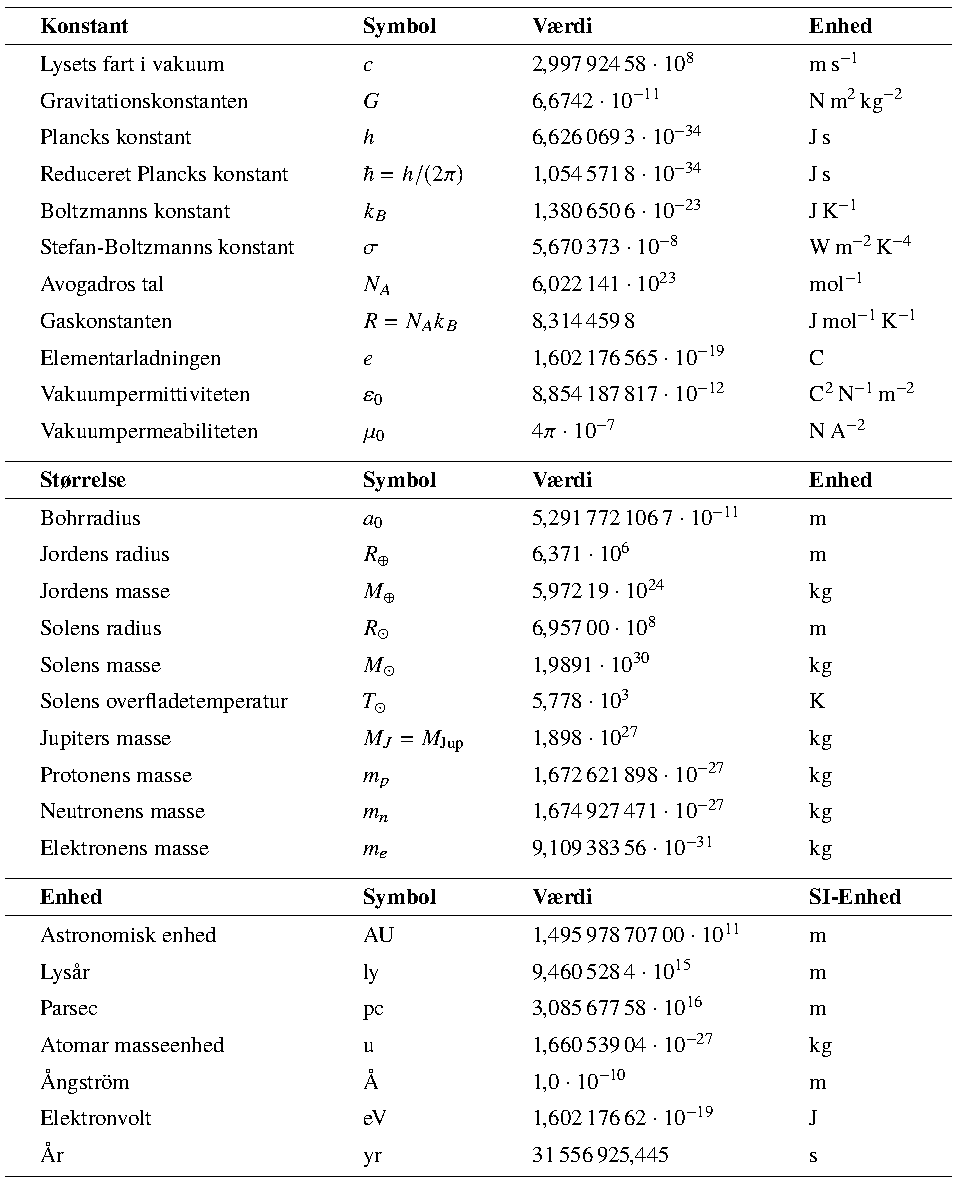
\includegraphics[width = 0.92 \textwidth]{Mat/matfig/Konstanter.pdf}
    \label{fysiske_konstanter}
\end{figure}

